\documentclass[a4paper, 11pt]{article}
\usepackage[utf8]{inputenc}
\usepackage[T1]{fontenc}
\usepackage{graphicx}
\usepackage{fancyhdr}
\pagestyle{fancy}
\usepackage{lastpage}

\fancyfoot[C]{Rapport en \LaTeX:\\
\textbf{Page \thepage/\pageref{LastPage}}}
\fancyfoot[R]{\today}

\title{Rapport du Jeu d’infection}
\author{Pierre Maurand - 21702704}
\date{18 février 2019}

\begin{document}

\maketitle

\thispagestyle{empty}
\setcounter{page}{0}

\newpage
\tableofcontents
\newpage

\section{Expérimentations}
\subsection{Consignes}
\hspace{\parindent}
En considérant que la profondeur de raisonnement est la même pour les deux adversaires et en fixant la taille de la grille, tracez des courbes représentant le nombre de nœuds explorés par MinMax puis AlphaBeta selon la profondeur de raisonnement.\\

Puis, identifiez l’intérêt du raisonnement en profondeur par rapport à des coups d’avances. Fixez une taille de grille et une profondeur de raisonnement pour les deux joueurs. Expérimentez en donnant des coups d’avance au joueur blanc et en augmentant la profondeur pour le joueur noir. Indiquez dans un tableau à deux dimensions (coups d’avance du joueur blanc, surplus de profondeur du joueur noir) si le joueur noir gagne ou perd.

\subsection{Résultat}
\hspace{\parindent}
D'après les expérimentations sur le nombre de branches visités par le MinMax et l'AlphaBeta, on peut clairement voir que plus la profondeur est importante, plus le nombre de branches a visité croit de façon exponentielle. Mais on remarque aussi très bien la logique de l'AlphaBeta de ne pas visiter toutes les branches, ce qui permet de gagner beaucoup de temps en visitant moins de branches.\\

Voici des graphes réalisés avec des combats entre des MinMax et des combats entre des AlphaBeta, le résultat est pratiquement similaire sur de petites profondeur, mais le MinMax restera le plus coûteux car il monte exponentiellement bien plus vite que l'Alphabeta :\\

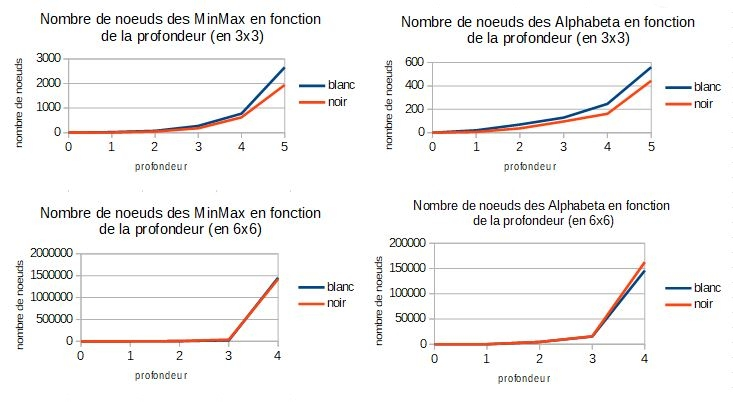
\includegraphics[scale=0.5]{images/illu1.png}\\

L'image précédente illustre très bien cette différence entre l'AlphaBeta et le MinMax. On ne la remarque d'abord pas pour une profondeur de 1 car ils sont alors identiques, puis viens une augmentation de quelques milliers de passages, qui se transforme vite en quelques millions après une petite augmentation de la profondeur sûr de grande grille.\\

L'intérêt du raisonnement en profondeur permet d'aller une idée de toutes les situations possibles ce qui augmente le nombre de banches à visité, tandis que avec un élagage, nous visons un score maximal en laissant de côté les branches pour lesquels il n'est pas intéressant de visité toutes les branches.\\

Les deux méthodes sont alors identiques, mais l'élagage de l'AlphaBeta permet une optimisation de la méthode de recherche du meilleur coup et donc d'aller plus loin en profondeur, ce qui est une stratégie plutôt efficace puisque nos deux programmes fond la même chose.\\

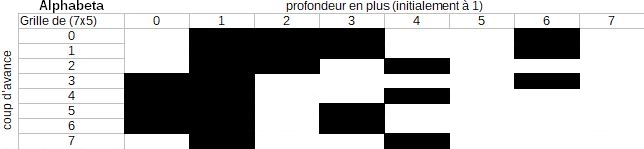
\includegraphics[scale=0.5]{images/illu2.png}\\
\newline

Cette image nous montre l'expérimentation de plusieurs parties réalisées sur une grille de 7x5 et une profondeur initiale de 1, avec un élagage pour aller plus loin dans la recherche (sachant que les résultat seront identique pour un MinMax). Plus le coups d'avance est important pour le joueur blanc, plus il faudras en profondeur pour le joueur noir pour gagner et inversement.\\

\end{document}
